\documentclass[9pt]{extarticle}
\usepackage[T1]{fontenc}
\usepackage[spanish,es-noquoting]{babel}
\usepackage[letterpaper,top=2.5cm,bottom=2.5cm,left=68.5pt,right=53.85pt]{geometry}
\usepackage{enumitem}
\setlist[enumerate]{leftmargin=-2.5pt,labelsep=5pt}
\usepackage{amsmath,amssymb}
\usepackage{graphicx}
\setlength{\parindent}{0pt}
\setlength{\parskip}{0.8ex}
\setlength{\fboxsep}{3.5pt}

\begin{document}

{\huge\textbf{Universidad de Buenos Aires}}\\[14.1pt]
{\huge\textbf{Laboratorio de Sistemas Embebidos}}\\[14.1pt]
{\huge\textbf{Especialización en Inteligencia Artificial}}

\vspace{2ex}\vspace{3.5pt}
\textbf{Análisis de Series de Tiempo 1}

\vspace{1.5ex}\vspace{5.3pt}
\textbf{Docente}: Camilo Argoty

\vspace{1ex}\vspace{7.1pt}
\hspace*{35pt}\fbox{\begin{minipage}{396pt}
\vspace{0.5ex}
Nombre:\qquad Franco Marcelo Morero \qquad Código:\qquad a2533\\[8.5pt]
Fecha: \underline{\makebox[5cm][l]{\ 31 de octubre de 2026}}
\vspace{0.3ex}
\end{minipage}}

\vspace{2ex}\vspace{-3.3pt}
\begin{center}\hspace*{-15pt}\textbf{PRIMER TRABAJO PRÁCTICO}\end{center}\vspace{-5.7pt}

%% ---------------------------------------------------------------- Ejercicio 1
\begin{enumerate}
\item (4 puntos) Sea:
\[ Y_t = R\cos(2\pi(ft+\Phi)) \]
una serie de tiempo, donde $R$ y $\Phi$ son variables aleatorias independientes y $f$ es una frecuencia fija. La fase $\Phi$ se distribuye uniforme sobre el intervalo $(0,1)$, mientras que la amplitud $R$ tiene una distribución de Rayleigh con densidad $f(r) = re^{-r^2/2}$ para $r>0$. Muestre que, para todo $t$, $Y_t$ tiene una distribución normal.\\
Pista: Defina $X = R\sin(2\pi(ft+\Phi))$ y $Y = R\cos(2\pi(ft+\Phi))$ y utilice la relación $X^2+Y^2=R^2$ para calcular la densidad conjunta de $(X,Y)$ a partir de la densidad conjunta de $(R,\Phi)$.
\end{enumerate}

\hrulefill

Tenemos la serie de tiempo
\[
Y_t = R\cos\bigl(2\pi(ft+\Phi)\bigr)
\]
donde $R$ y $\Phi$ son independientes, $f$ es una frecuencia fija, $\Phi \sim U(0,1)$ y $R \sim \text{Rayleigh}$.

Usemos $x^2+y^2=R^2$. Definimos
\begin{align*}
X &= R\sin\bigl(2\pi(ft+\Phi)\bigr)\\
Y &= R\cos\bigl(2\pi(ft+\Phi)\bigr)
\end{align*}
es decir, $R$ es un radio y $2\pi(ft+\Phi)$ un ángulo.

Como $R$ y $\Phi$ son independientes, su densidad conjunta es el producto de las marginales
\[
f_{R,\Phi}(r,\phi) = f_R(r)\, f_\Phi(\phi)
\]
donde, por enunciado,
\[
f_R(r) = r\,e^{-r^2/2} \quad (r>0)
\qquad\qquad
f_\Phi(\phi) = 1 \quad (0<\phi<1)
\]
Entonces
\[
f_{R,\Phi}(r,\phi) = r\,e^{-r^2/2}, \qquad r>0,\ 0<\phi<1
\]

Ahora para calcular la densidad $f_{X,Y}(x,y)$ usamos la fórmula que vimos en probabilidad para transformación de variable
\[
f_{X,Y}(x,y) = f_{R,\Phi}\bigl(r(x,y),\phi(x,y)\bigr)\,\lvert \det J\rvert
\]
donde $J$ es el jacobiano de la transformación inversa
\[
J = \begin{pmatrix}
\dfrac{\partial r}{\partial x} & \dfrac{\partial r}{\partial y}\\[2ex]
\dfrac{\partial \phi}{\partial x} & \dfrac{\partial \phi}{\partial y}
\end{pmatrix}
\]

Sabemos que $R^2 = x^2+y^2$, entonces como $r>0$
\[
\boxed{r = \sqrt{x^2+y^2}}
\]
Por lo que
\begin{alignat*}{2}
\frac{\partial r}{\partial x} &= \frac{1}{2}(x^2+y^2)^{-1/2}\,2x
&\qquad\Rightarrow\qquad &\boxed{\frac{\partial r}{\partial x} = \frac{x}{\sqrt{x^2+y^2}}}\\
\frac{\partial r}{\partial y} &= \frac{1}{2}(x^2+y^2)^{-1/2}\,2y
&\qquad\Rightarrow\qquad &\boxed{\frac{\partial r}{\partial y} = \frac{y}{\sqrt{x^2+y^2}}}
\end{alignat*}

Ahora para $\phi$ tenemos que
\begin{align*}
x &= r\sin\bigl(2\pi(ft+\phi)\bigr)\\
y &= r\cos\bigl(2\pi(ft+\phi)\bigr)
\end{align*}
Si tomamos $x/y$ vemos que
\begin{align*}
\frac{x}{y} &= \frac{r\sin\bigl(2\pi(ft+\phi)\bigr)}{r\cos\bigl(2\pi(ft+\phi)\bigr)}\\
\frac{x}{y} &= \tan\bigl(2\pi(ft+\phi)\bigr)\\
\tan^{-1}(x/y) &= 2\pi(ft+\phi)\\
\frac{\tan^{-1}(x/y)}{2\pi} &= ft+\phi
\end{align*}
\[
\boxed{\phi = \frac{1}{2\pi}\arctan(x/y) - ft}
\]

Busquemos ahora $\dfrac{\partial\phi}{\partial x}$ y $\dfrac{\partial\phi}{\partial y}$. Tenemos que
\[
\frac{d}{dx}\arctan(u) = \frac{u'}{1+u^2}
\qquad
\frac{\partial}{\partial x}\frac{x}{y} = \frac{1}{y}\,;\quad
\frac{\partial}{\partial y}\frac{x}{y} = -\frac{x}{y^2}
\]
Luego
\begin{align*}
\frac{\partial}{\partial x}\arctan(x/y)
&= \frac{1/y}{1+(x/y)^2} = \frac{1/y}{1+x^2/y^2}
= \frac{1/y}{\frac{y^2+x^2}{y^2}} = \frac{y}{y^2+x^2}\\
\frac{\partial}{\partial y}\arctan(x/y)
&= \frac{-x/y^2}{\frac{y^2+x^2}{y^2}} = \frac{-x}{y^2+x^2}
\end{align*}
Por lo que
\[
\boxed{\frac{\partial\phi}{\partial x} = \frac{1}{2\pi}\,\frac{y}{x^2+y^2}}
\qquad
\boxed{\frac{\partial\phi}{\partial y} = \frac{1}{2\pi}\,\frac{-x}{x^2+y^2}}
\]

Ahora veamos $J$
\[
J = \begin{pmatrix}
\dfrac{\partial r}{\partial x} & \dfrac{\partial r}{\partial y}\\[2ex]
\dfrac{\partial \phi}{\partial x} & \dfrac{\partial \phi}{\partial y}
\end{pmatrix}
= \begin{bmatrix}
\dfrac{x}{\sqrt{x^2+y^2}} & \dfrac{y}{\sqrt{x^2+y^2}}\\[2ex]
\dfrac{y}{2\pi(x^2+y^2)} & \dfrac{-x}{2\pi(x^2+y^2)}
\end{bmatrix}
\]
Luego
\begin{align*}
\det(J) &= \left[\frac{x}{\sqrt{x^2+y^2}}\cdot\frac{-x}{2\pi(x^2+y^2)}\right]
- \left[\frac{y}{\sqrt{x^2+y^2}}\cdot\frac{y}{2\pi(x^2+y^2)}\right]\\
&= \frac{-x^2}{2\pi(x^2+y^2)^{3/2}} - \frac{y^2}{2\pi(x^2+y^2)^{3/2}}\\
&= \frac{-(x^2+y^2)}{2\pi(x^2+y^2)^{3/2}}\\
&= -\frac{1}{2\pi\sqrt{x^2+y^2}}
\end{align*}
\[
\therefore\quad \boxed{\lvert\det(J)\rvert = \frac{1}{2\pi\sqrt{x^2+y^2}}}
\]

Luego, utilizando todo lo obtenido
\begin{align*}
f_{R,\Phi}\bigl(r(x,y),\phi(x,y)\bigr) &= \sqrt{x^2+y^2}\;e^{-\frac{\left(\sqrt{x^2+y^2}\right)^2}{2}}\\
&\boxed{f_{R,\Phi}\bigl(r(x,y),\phi(x,y)\bigr) = \sqrt{x^2+y^2}\;e^{-\frac{x^2+y^2}{2}}}
\end{align*}
porque $f_{R,\Phi}(r,\phi) = r\,e^{-r^2/2}$ y $r=\sqrt{x^2+y^2}$.

Entonces
\begin{align*}
f_{X,Y}(x,y) &= f_{R,\Phi}\bigl(r(x,y),\phi(x,y)\bigr)\cdot\lvert\det J\rvert\\
&= \sqrt{x^2+y^2}\;e^{-\frac{x^2+y^2}{2}}\cdot\frac{1}{2\pi\sqrt{x^2+y^2}}\\
&= \frac{1}{2\pi}\,e^{-\frac{x^2+y^2}{2}}
\end{align*}
\[
\therefore\quad \boxed{f_{X,Y}(x,y) = \frac{1}{2\pi}\,e^{-\frac{x^2+y^2}{2}}}
\]

Ahora nos falta la densidad marginal de $Y$
\begin{align*}
f_Y(y) &= \int_{-\infty}^{\infty} f_{X,Y}(x,y)\,dx\\
&= \int_{-\infty}^{\infty} \frac{1}{2\pi}\,e^{-\frac{x^2+y^2}{2}}\,dx\\
&= \frac{1}{2\pi}\,e^{-y^2/2}\int_{-\infty}^{\infty} e^{-x^2/2}\,dx
\end{align*}
Resolvamos la integral gaussiana. Recordamos que la densidad de una normal estándar $Z \sim N(0,1)$ es
\[
f_Z(x) = \frac{1}{\sqrt{2\pi}}\,e^{-x^2/2}
\]
y sabemos que la función de densidad de probabilidad integra 1 sobre su dominio. Por lo que
\begin{align*}
\int_{-\infty}^{\infty}\frac{1}{\sqrt{2\pi}}\,e^{-x^2/2}\,dx &= 1\\
\int_{-\infty}^{\infty} e^{-x^2/2}\,dx &= \sqrt{2\pi}
\end{align*}
Ahora volvemos a nuestro problema
\begin{align*}
f_Y(y) &= \frac{1}{2\pi}\,e^{-y^2/2}\int_{-\infty}^{\infty} e^{-x^2/2}\,dx\\
&= \frac{1}{2\pi}\,e^{-y^2/2}\,\sqrt{2\pi}
\end{align*}
\[
\boxed{f_Y(y) = \frac{1}{\sqrt{2\pi}}\,e^{-\frac{y^2}{2}}}
\]
que si la comparamos con una normal
\[
f(y) = \frac{1}{\sigma\sqrt{2\pi}}\,e^{-\frac{(y-\mu)^2}{2\sigma^2}}
\]
vemos que la media es $\mu=0$ y la varianza $\sigma^2=1$. Por lo que
\[
\boxed{Y_t \sim N(0,1)\quad \forall t}
\]

%% ---------------------------------------------------------------- Ejercicio 2
\bigskip
\hrule
\bigskip
\begin{enumerate}\setcounter{enumi}{1}
\item (3 puntos) Sea:
\[ Y_t = \mu + \varepsilon_t + \varepsilon_{t-1} \]
donde $\varepsilon_t$ es un ruido blanco de media 0.\\
Sea
\[ \bar{Y} = \frac{1}{n}\sum_{t=1}^{n} Y_t \]
Encuentre $Var(\bar{Y})$
\end{enumerate}

\hrulefill

Tenemos
\[
Y_t = \mu + \varepsilon_t + \varepsilon_{t-1}
\]
donde $\varepsilon_t$ es ruido blanco de media cero. Para ruido blanco sabemos que
\begin{align*}
E(\varepsilon_t) &= 0\\
\operatorname{Var}(\varepsilon_t) &= \sigma^2\\
\operatorname{Cov}(\varepsilon_t,\varepsilon_s) &= 0, \quad t \neq s
\end{align*}
y tenemos el promedio muestral
\begin{align*}
\bar{Y} &= \frac{1}{n}\sum_{t=1}^{n} Y_t\\
&= \frac{1}{n}\sum_{t=1}^{n}\left(\mu + \varepsilon_t + \varepsilon_{t-1}\right)\\
&= \frac{1}{n}\left[\sum_{t=1}^{n}\mu + \sum_{t=1}^{n}\varepsilon_t + \sum_{t=1}^{n}\varepsilon_{t-1}\right]\\
&= \frac{1}{n}\left[n\mu + \sum_{t=1}^{n}\varepsilon_t + \sum_{t=1}^{n}\varepsilon_{t-1}\right]\\
&= \mu + \frac{1}{n}\left[\sum_{t=1}^{n}\varepsilon_t + \sum_{t=1}^{n}\varepsilon_{t-1}\right]
\end{align*}
Recordando las propiedades de la varianza
\begin{align*}
\operatorname{Var}(X+c) &= \operatorname{Var}(X)\\
\operatorname{Var}(aX) &= a^2\operatorname{Var}(X)\\
\operatorname{Var}(A+B) &= \operatorname{Var}(A)+\operatorname{Var}(B)+2\operatorname{Cov}(A,B)
\end{align*}
vemos que
\begin{align*}
\operatorname{Var}(\bar{Y}) &= \operatorname{Var}\left[\mu + \frac{1}{n}\left(\sum_{t=1}^{n}\varepsilon_t + \sum_{t=1}^{n}\varepsilon_{t-1}\right)\right]\\
&= \frac{1}{n^2}\operatorname{Var}\left[\sum_{t=1}^{n}\varepsilon_t + \sum_{t=1}^{n}\varepsilon_{t-1}\right]\\
&= \frac{1}{n^2}\left[\operatorname{Var}\left(\sum_{t=1}^{n}\varepsilon_t\right) + \operatorname{Var}\left(\sum_{t=1}^{n}\varepsilon_{t-1}\right) + 2\operatorname{Cov}\left(\sum_{t=1}^{n}\varepsilon_t, \sum_{t=1}^{n}\varepsilon_{t-1}\right)\right]
\end{align*}
Luego, como los términos de ruido blanco no están correlacionados,
\[
\boxed{\operatorname{Var}\left(\sum_{t=1}^{n}\varepsilon_t\right) = n\sigma^2}
\qquad
\boxed{\operatorname{Var}\left(\sum_{t=1}^{n}\varepsilon_{t-1}\right) = n\sigma^2}
\]
Luego, para la covarianza de las sumatorias, tomamos
\begin{align*}
A &= \varepsilon_1 + \varepsilon_2 + \dots + \varepsilon_n\\
B &= \varepsilon_0 + \varepsilon_1 + \dots + \varepsilon_{n-1}
\end{align*}
Hay que tener en cuenta al calcular $\operatorname{Cov}(A,B)$ que solo contribuyen a la covarianza los términos que aparecen en ambas sumatorias, porque
\[
\operatorname{Cov}(\varepsilon_i,\varepsilon_j) =
\begin{cases}
\sigma^2 & i = j\\
0 & i \neq j
\end{cases}
\]
Vemos que $A$ y $B$ comparten todos los términos menos el último de $A$ ($\varepsilon_n$) y el primero de $B$ ($\varepsilon_0$), entonces comparten $n-1$ términos. Por lo que
\[
\boxed{\operatorname{Cov}(A,B) = (n-1)\sigma^2}
\]
Ahora, reemplazando en la fórmula original,
\begin{align*}
\operatorname{Var}(\bar{Y}) &= \frac{1}{n^2}\left[n\sigma^2 + n\sigma^2 + 2(n-1)\sigma^2\right]\\
&= \frac{1}{n^2}\,\sigma^2\left[n + n + 2(n-1)\right]\\
&= \frac{1}{n^2}\,\sigma^2\,(2n + 2n - 2)
\end{align*}
\[
\boxed{\operatorname{Var}(\bar{Y}) = \frac{4n-2}{n^2}\,\sigma^2}
\]

%% ---------------------------------------------------------------- Ejercicio 3
\bigskip
\hrule
\bigskip
\begin{enumerate}\setcounter{enumi}{2}
\item (3 puntos) Sea:
\[ Y_t = -10 + (0)\varepsilon_t + (-7)\varepsilon_{t-1} + (-8)\varepsilon_{t-2} \]
Encuentre la función de autocorrelación de $Y_t$.
\end{enumerate}

\hrulefill

Tenemos
\[
Y_t = -10 + (0)\varepsilon_t + (-7)\varepsilon_{t-1} + (-8)\varepsilon_{t-2}
\]
o sea
\[
Y_t = -10 - 7\varepsilon_{t-1} - 8\varepsilon_{t-2}
\]

Queremos calcular la ACF
\[
\rho(h) = \frac{\gamma(h)}{\gamma(0)}
\]
donde
\begin{align*}
\gamma(h) &= \operatorname{Cov}(Y_t, Y_{t-h}) \quad \text{es la autocovarianza para el rezago } h\\
\gamma(0) &= \operatorname{Var}(Y_t) \quad \text{es la varianza del proceso}
\end{align*}

Calculamos primero la media, recordando que el ruido blanco cumple
\begin{align*}
E(\varepsilon_t) &= 0\\
\operatorname{Var}(\varepsilon_t) &= \sigma^2\\
\operatorname{Cov}(\varepsilon_t, \varepsilon_s) &= 0, \quad t \neq s
\end{align*}
Entonces
\begin{align*}
E(Y_t) &= E[-10 - 7\varepsilon_{t-1} - 8\varepsilon_{t-2}]\\
&= -10 - 7\underbrace{E(\varepsilon_{t-1})}_{0} - 8\underbrace{E(\varepsilon_{t-2})}_{0}
\end{align*}
\[
\boxed{E(Y_t) = -10}
\]

Luego calculemos $\gamma(0)$
\begin{align*}
\gamma(0) &= \operatorname{Var}(Y_t)\\
&= \operatorname{Var}(-10 - 7\varepsilon_{t-1} - 8\varepsilon_{t-2})\\
&= \operatorname{Var}(-7\varepsilon_{t-1}) + \operatorname{Var}(-8\varepsilon_{t-2}) + \underbrace{2\operatorname{Cov}(-7\varepsilon_{t-1}; -8\varepsilon_{t-2})}_{0}\\
&= 49\sigma^2 + 64\sigma^2
\end{align*}
\[
\boxed{\gamma(0) = 113\sigma^2}
\]

Ahora veamos la autocovarianza en un rezago
\begin{align*}
\gamma(1) &= \operatorname{Cov}(Y_t, Y_{t-1})\\
Y_{t-1} &= -10 - 7\varepsilon_{t-2} - 8\varepsilon_{t-3}
\end{align*}
Para calcular la covarianza, las constantes no influyen y los términos de ruido blanco en distintos instantes tienen covarianza cero.
Vemos que el único término compartido es $\varepsilon_{t-2}$
\begin{align*}
Y_t &= -10 - 7\varepsilon_{t-1} \underline{- 8\varepsilon_{t-2}}\\
Y_{t-1} &= -10 \underline{- 7\varepsilon_{t-2}} - 8\varepsilon_{t-3}
\end{align*}
Entonces solo consideramos ese término al calcular la autocovarianza
\[
\gamma(1) = \operatorname{Cov}(-8\varepsilon_{t-2}; -7\varepsilon_{t-2})
\]
Usando la propiedad
\[
\operatorname{Cov}(aX, bY) = ab\operatorname{Cov}(X, Y)
\]
vemos que
\begin{align*}
\gamma(1) &= 56\operatorname{Cov}(\varepsilon_{t-2}; \varepsilon_{t-2})\\
&= 56\operatorname{Var}(\varepsilon_{t-2})
\end{align*}
\[
\boxed{\gamma(1) = 56\sigma^2}
\]

Veamos ahora qué pasa con $\gamma(2)$
\[
Y_{t-2} = -10 - 7\varepsilon_{t-3} - 8\varepsilon_{t-4}
\]
Vemos que $Y_{t-2}$ con $Y_t$ no comparten ningún término de ruido blanco, por lo que
\[
\boxed{\gamma(2) = 0}
\]
Luego vemos que pasa lo mismo para todo $h \geq 2$
\[
\boxed{\gamma(h) = 0 \quad \forall h \geq 2}
\]

Entonces tenemos
\begin{align*}
\gamma(0) &= 113\sigma^2\\
\gamma(1) &= 56\sigma^2\\
\gamma(h) &= 0, \quad \forall h \geq 2
\end{align*}
Luego calculamos $\rho(h) = \dfrac{\gamma(h)}{\gamma(0)}$ para 0, 1 y 2
\begin{align*}
\rho(0) &= \frac{\gamma(0)}{\gamma(0)} = 1\\
\rho(1) &= \frac{\gamma(1)}{\gamma(0)} = \frac{56\sigma^2}{113\sigma^2} = \frac{56}{113}\\
\rho(2) &= \frac{\gamma(2)}{\gamma(0)} = 0
\end{align*}
Entonces la función de autocorrelación de $Y_t$ es
\[
\boxed{
\rho(h) =
\begin{cases}
1 & h = 0\\[4pt]
\dfrac{56}{113} & |h| = 1\\[4pt]
0 & |h| \geq 2
\end{cases}
}
\]

Notemos que los rezagos negativos se incluyen porque la autocorrelación es simétrica, $\rho(-h) = \rho(h)$.

%% ---------------------------------------------------------------- Anexo
\clearpage
\begin{center}\textbf{Anexo: resolución manuscrita}\end{center}

\begin{center}
Ejercicio 1, página 1\\[1ex]
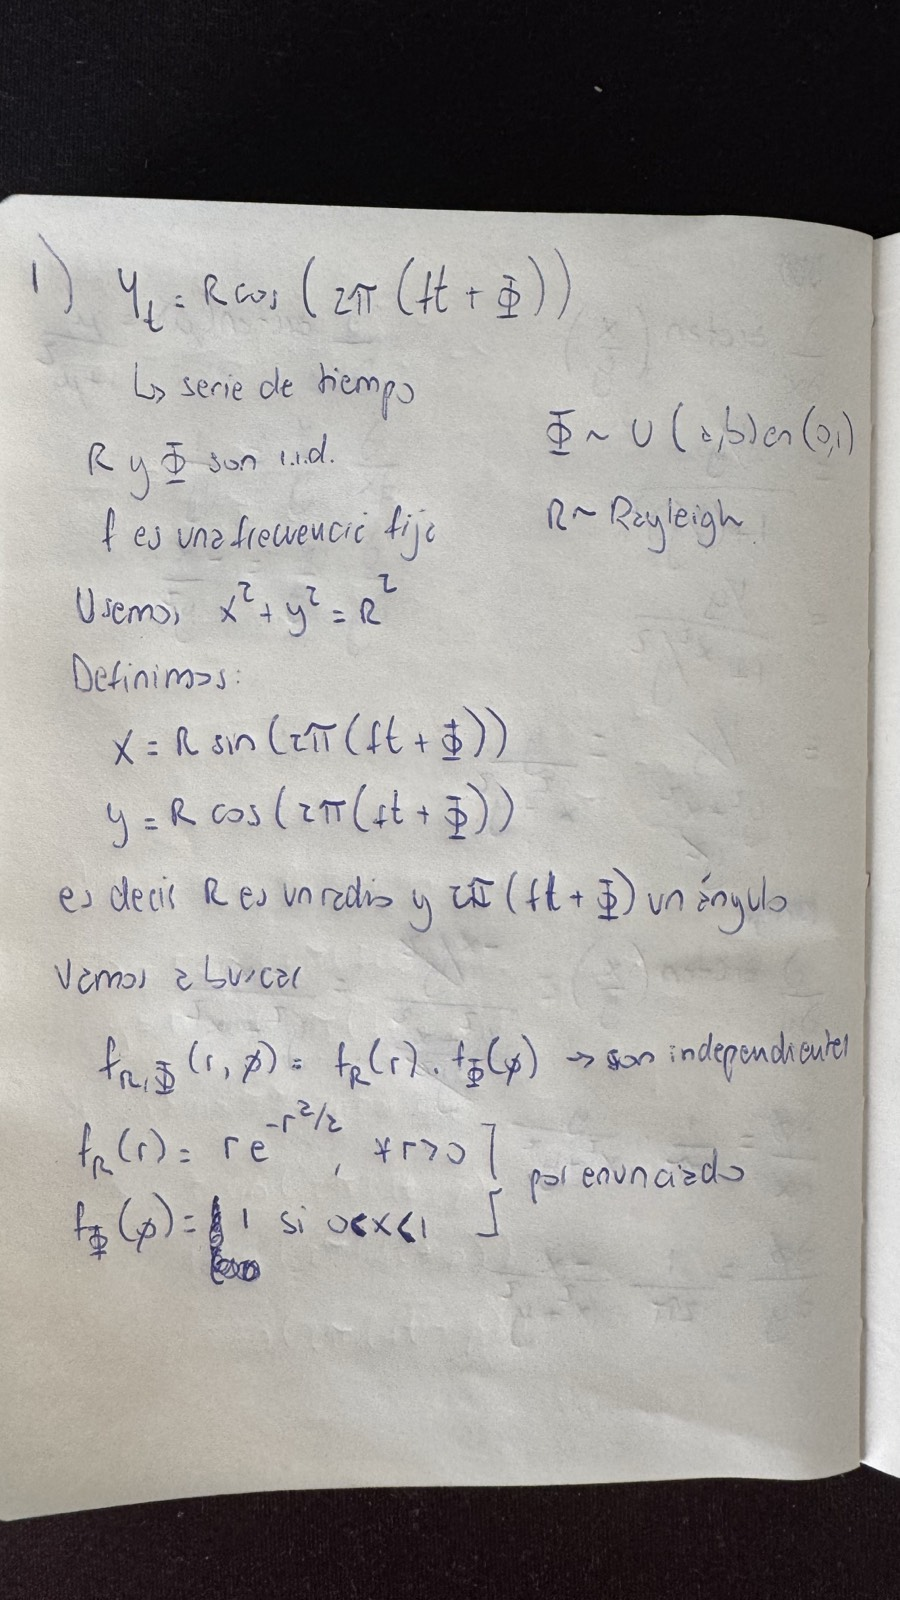
\includegraphics[height=0.86\textheight]{anexo/ej1_pag1.jpg}
\end{center}
\clearpage

\begin{center}
Ejercicio 1, página 2\\[1ex]
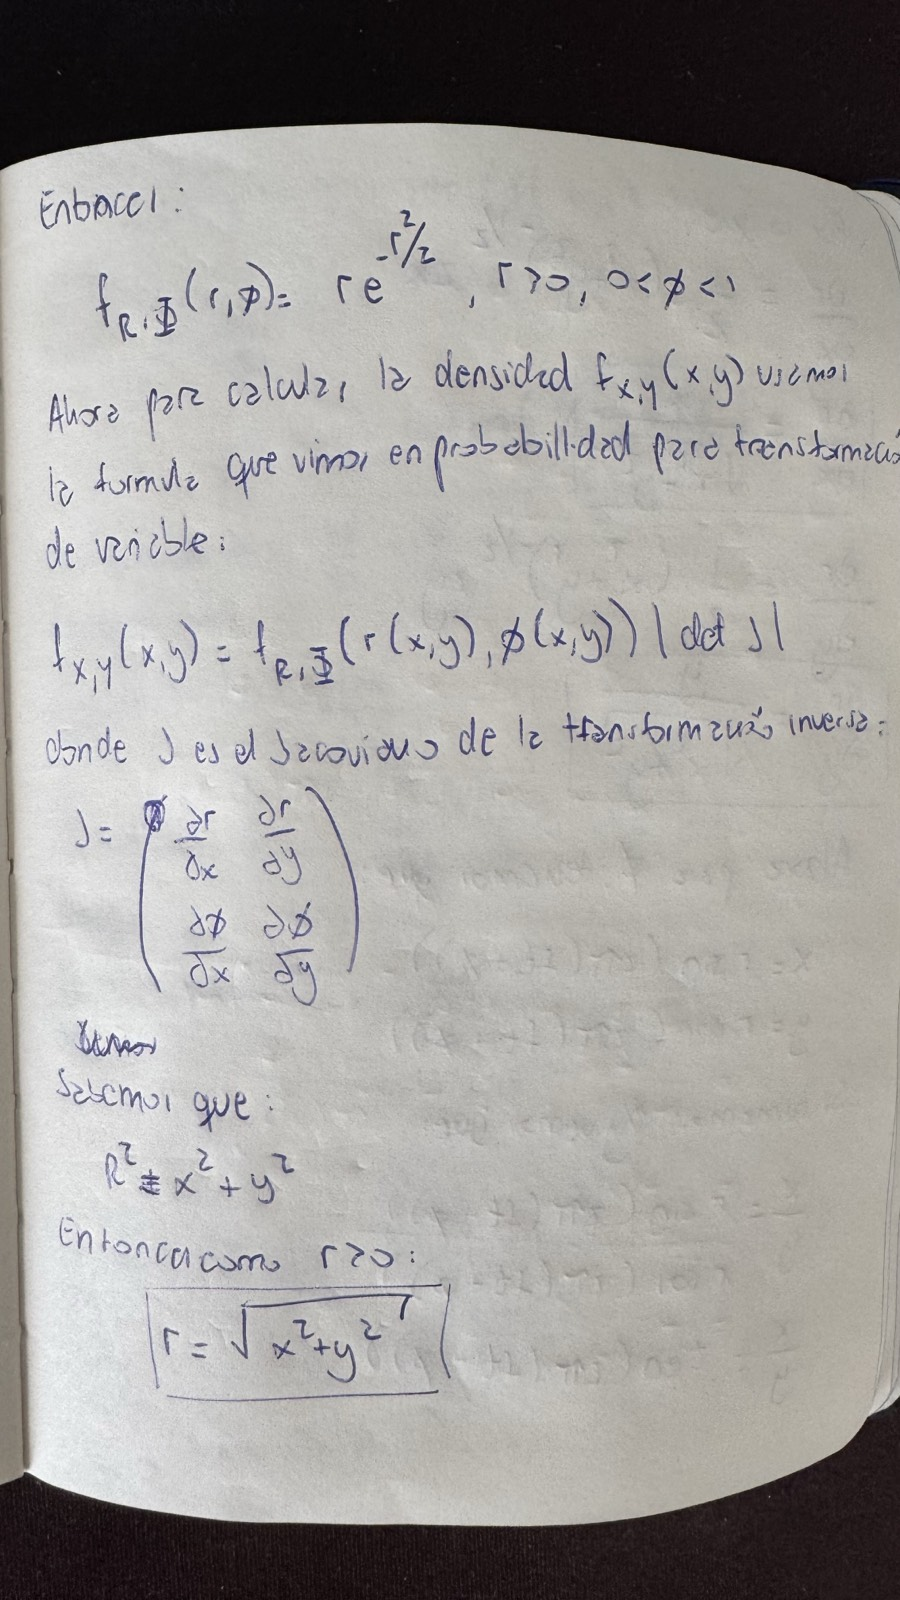
\includegraphics[height=0.86\textheight]{anexo/ej1_pag2.jpg}
\end{center}
\clearpage

\begin{center}
Ejercicio 1, página 3\\[1ex]
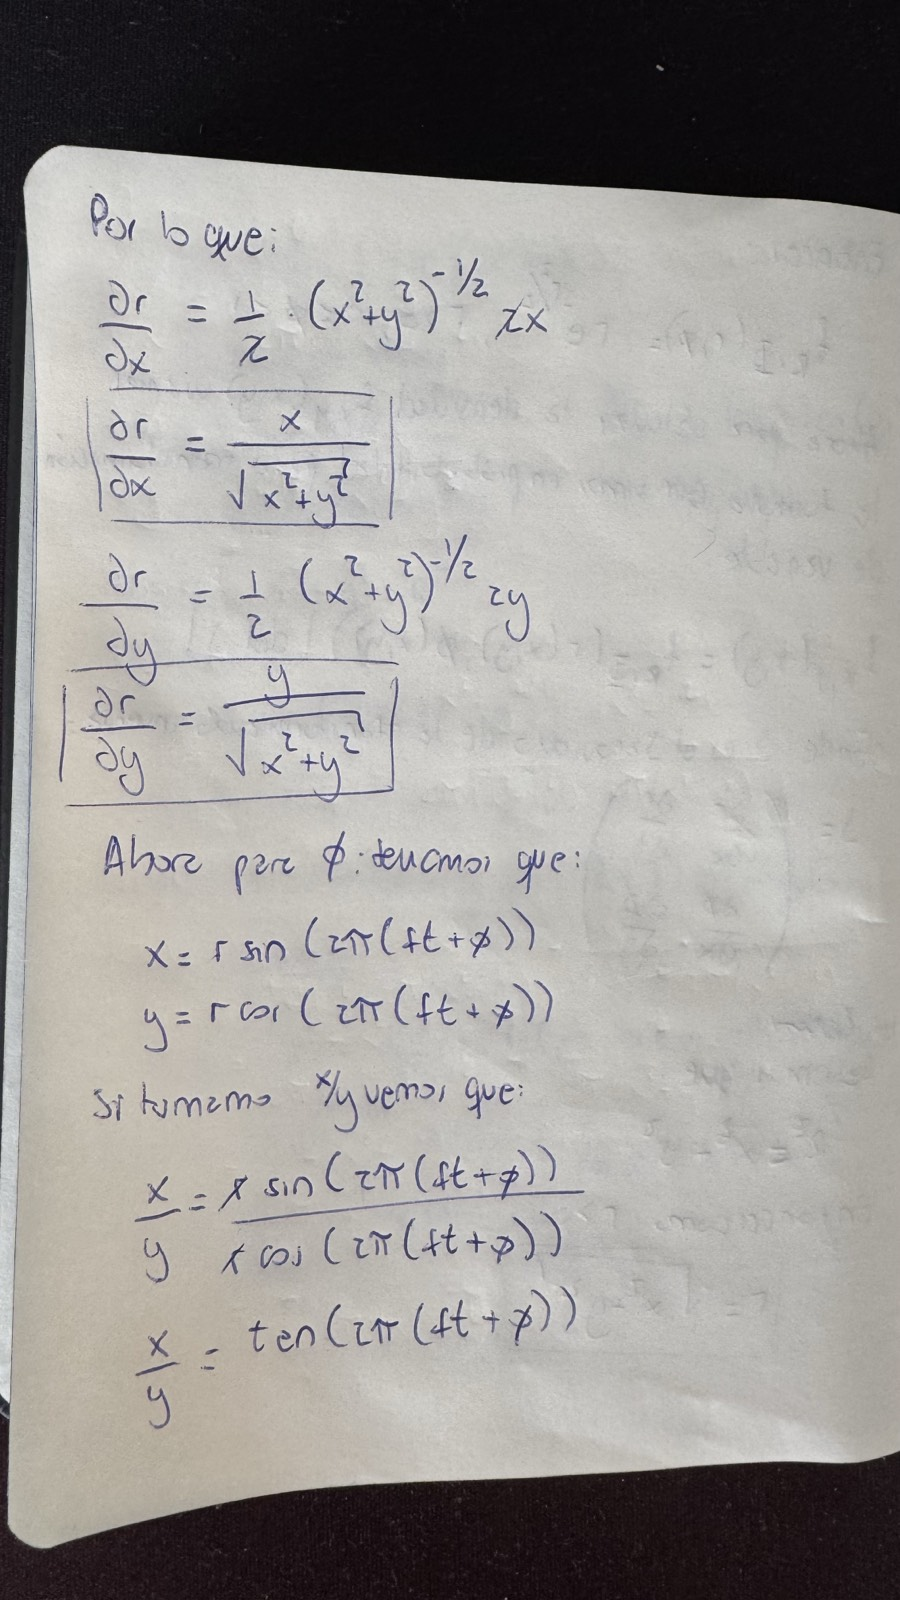
\includegraphics[height=0.86\textheight]{anexo/ej1_pag3.jpg}
\end{center}
\clearpage

\begin{center}
Ejercicio 1, página 4\\[1ex]
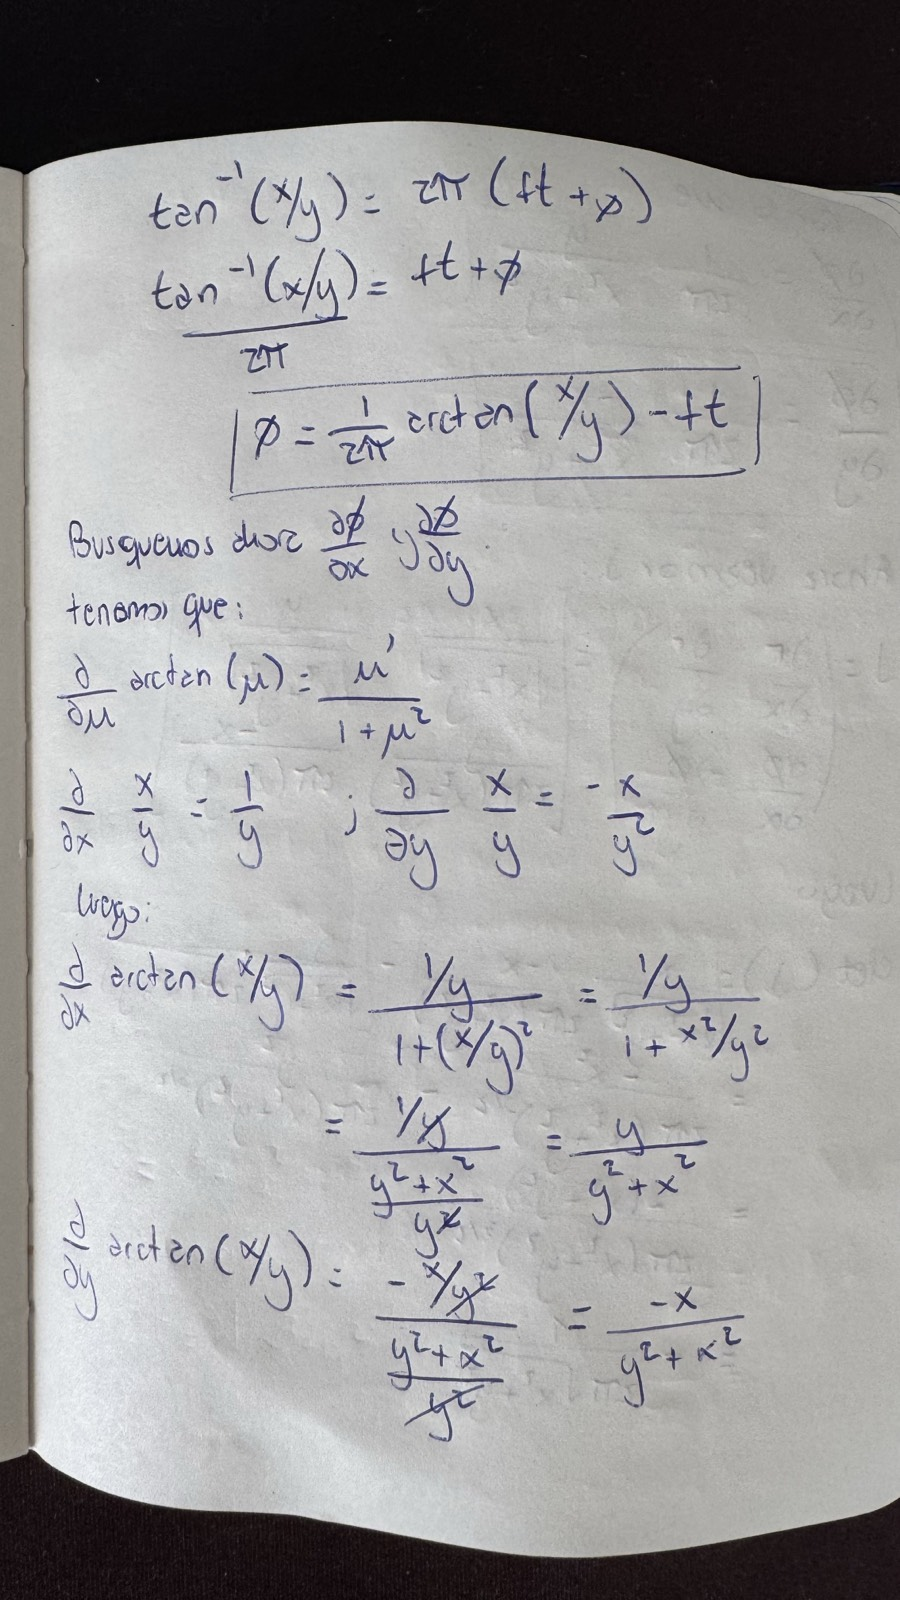
\includegraphics[height=0.86\textheight]{anexo/ej1_pag4.jpg}
\end{center}
\clearpage

\begin{center}
Ejercicio 1, página 5\\[1ex]
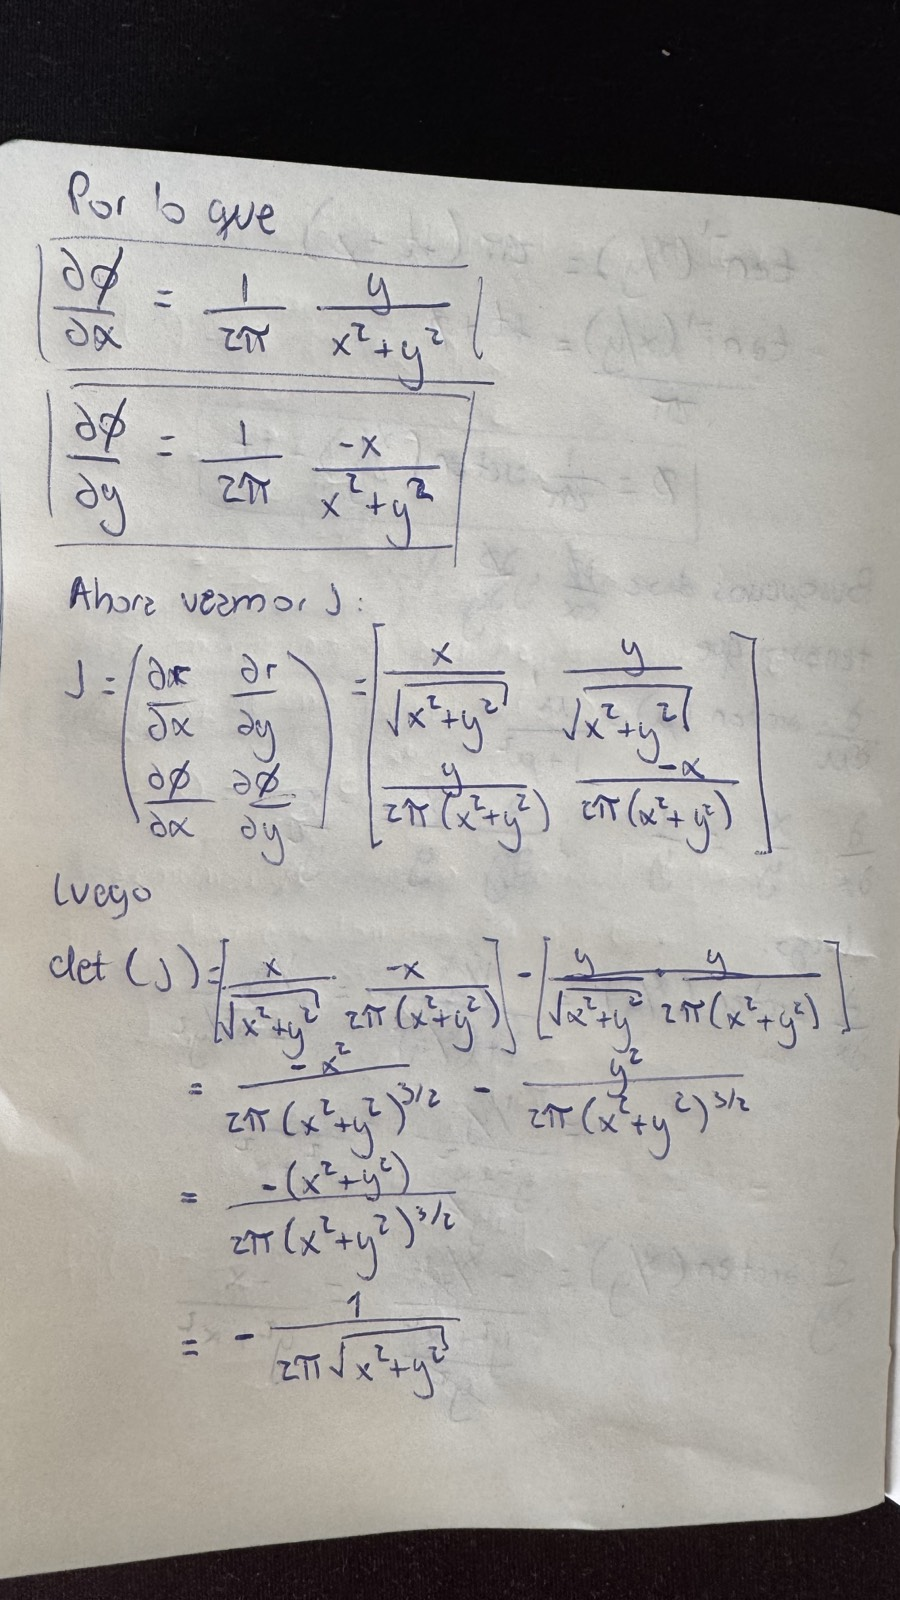
\includegraphics[height=0.86\textheight]{anexo/ej1_pag5.jpg}
\end{center}
\clearpage

\begin{center}
Ejercicio 1, página 6\\[1ex]
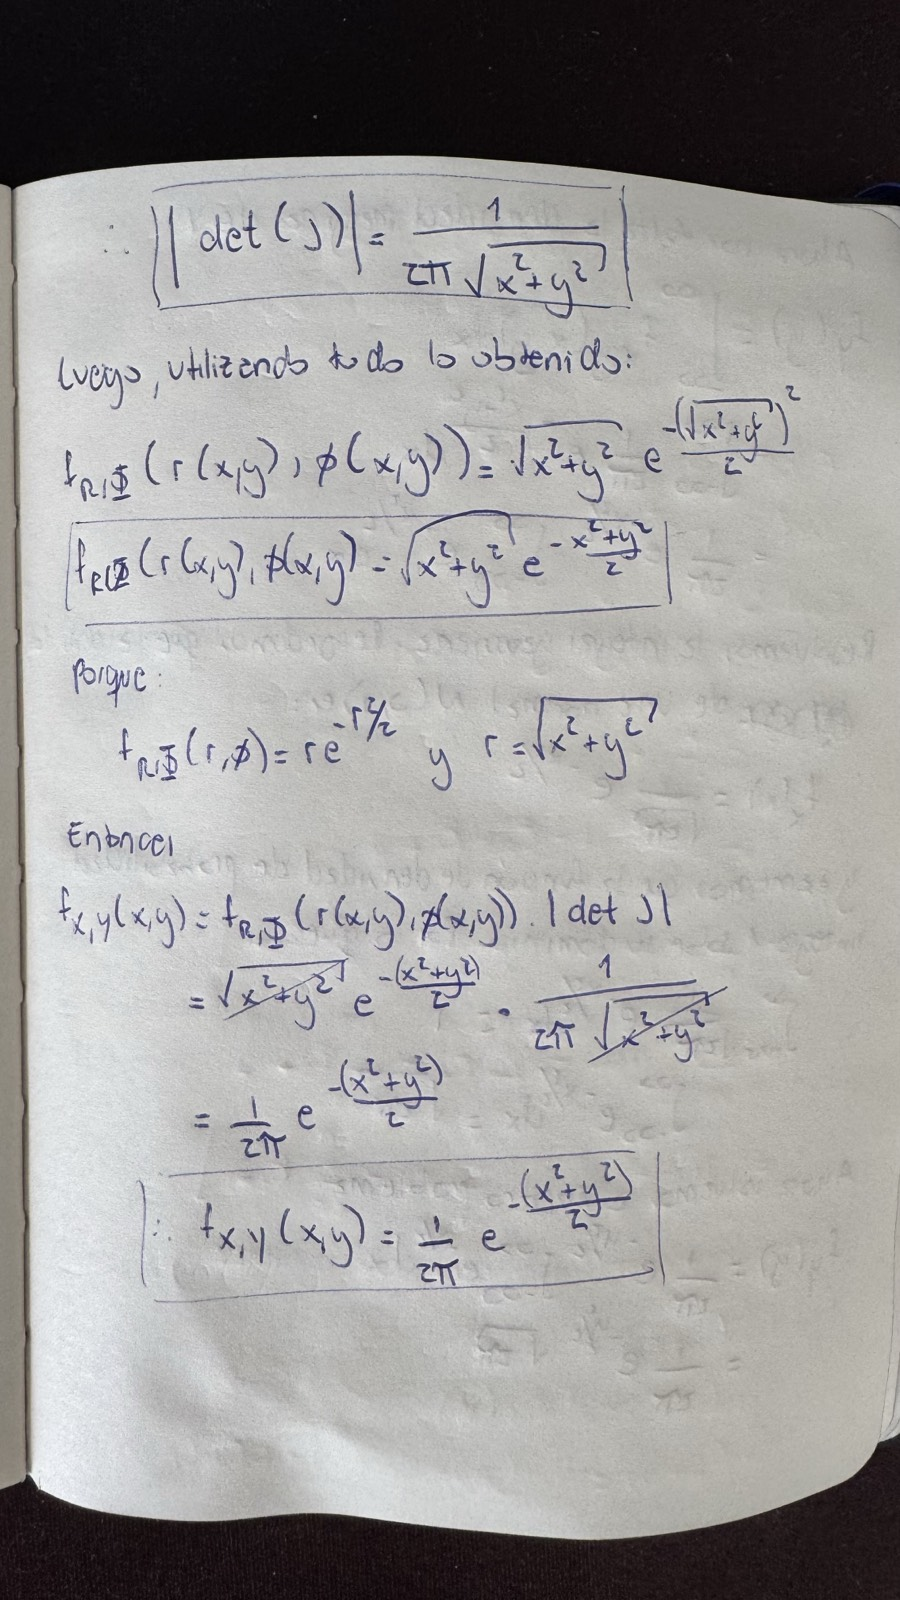
\includegraphics[height=0.86\textheight]{anexo/ej1_pag6.jpg}
\end{center}
\clearpage

\begin{center}
Ejercicio 1, página 7\\[1ex]
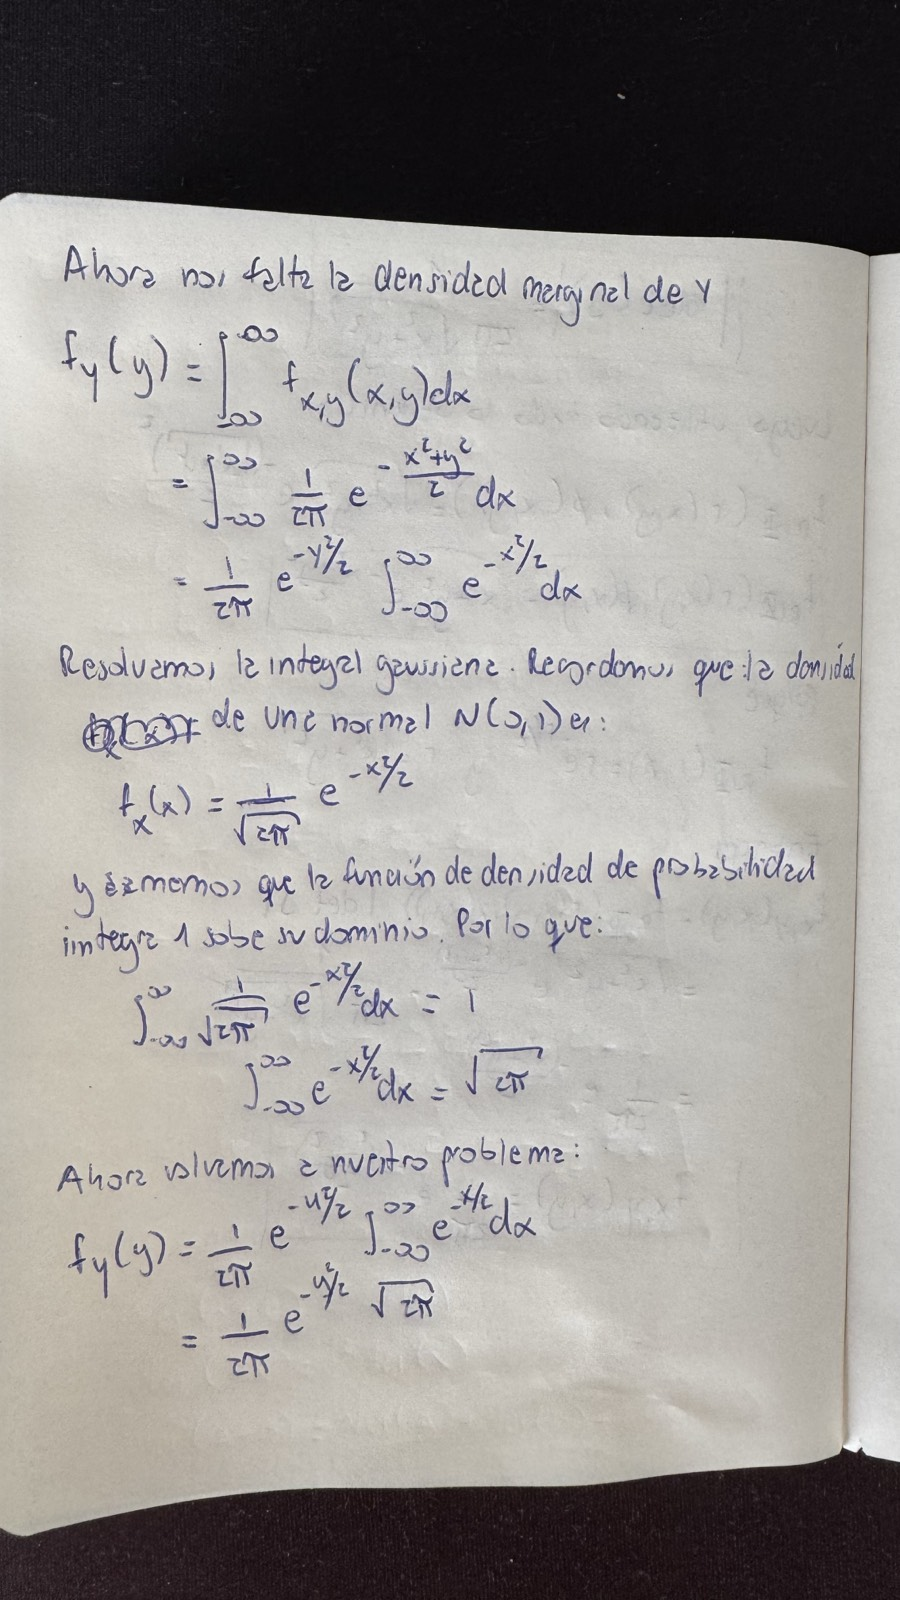
\includegraphics[height=0.86\textheight]{anexo/ej1_pag7.jpg}
\end{center}
\clearpage

\begin{center}
Ejercicio 1, página 8\\[1ex]
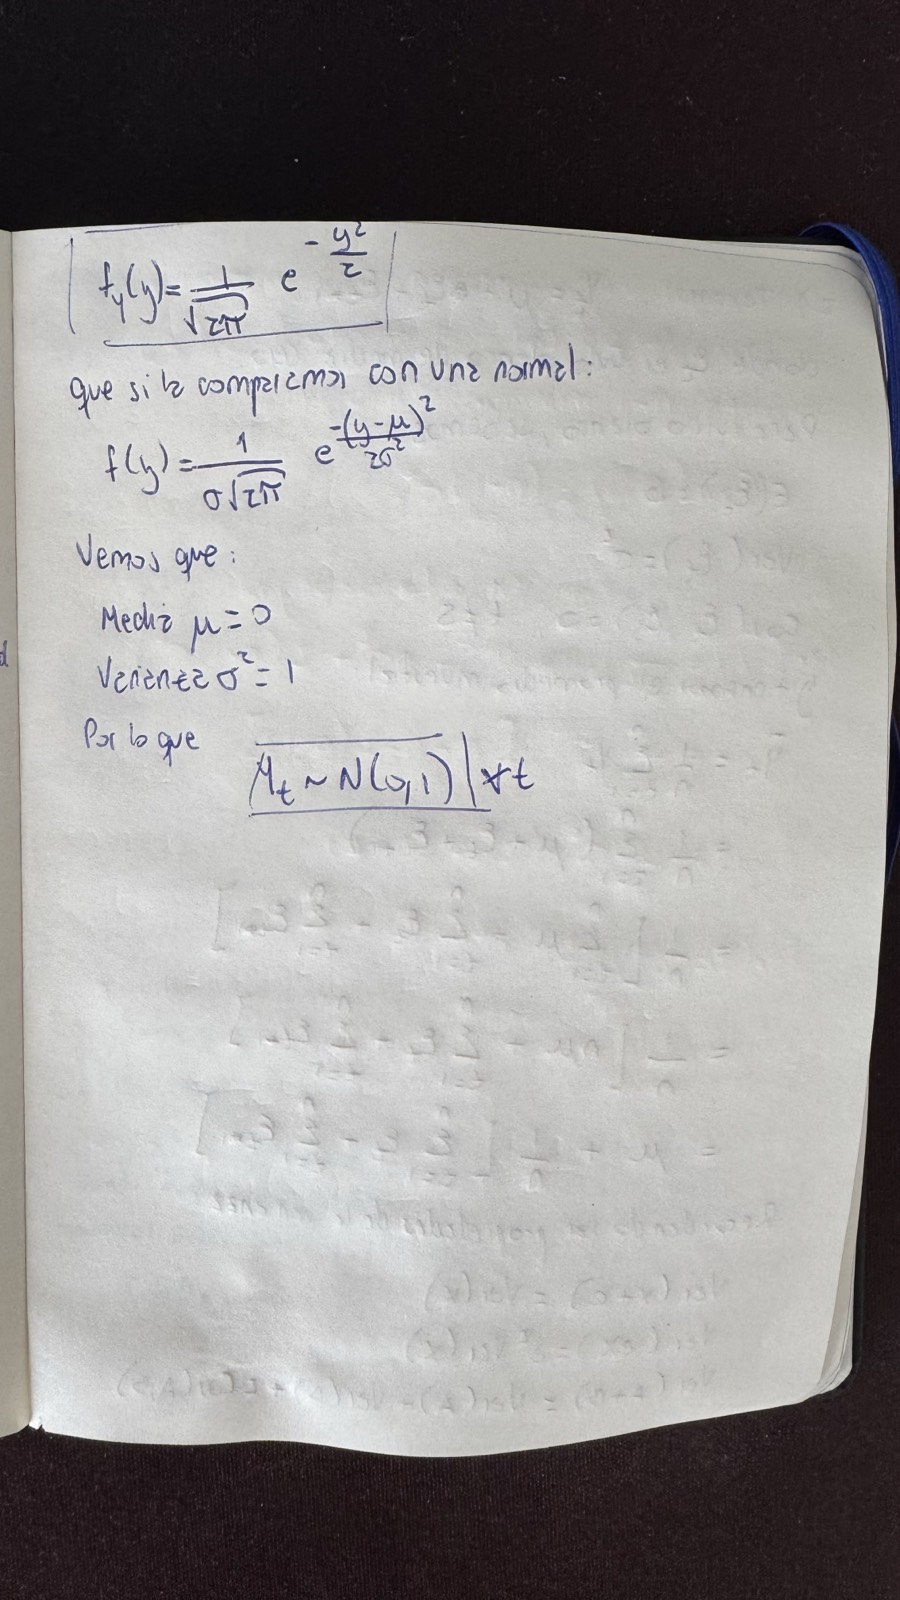
\includegraphics[height=0.86\textheight]{anexo/ej1_pag8.jpg}
\end{center}
\clearpage

\begin{center}
Ejercicio 2, página 1\\[1ex]
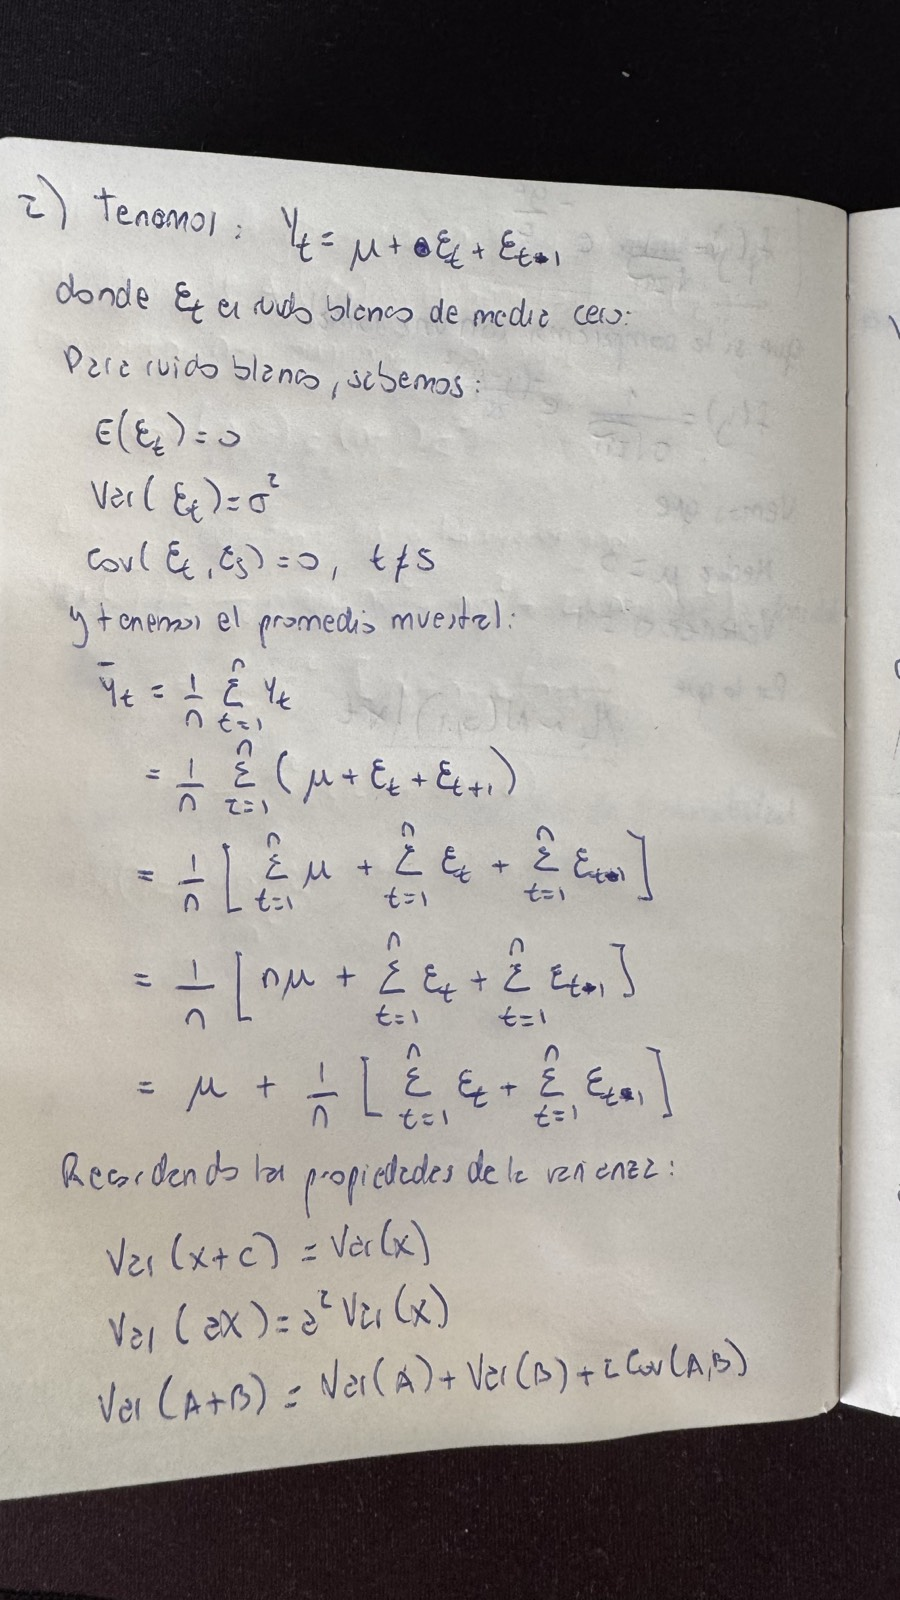
\includegraphics[height=0.86\textheight]{anexo/ej2_pag1.jpg}
\end{center}
\clearpage

\begin{center}
Ejercicio 2, página 2\\[1ex]
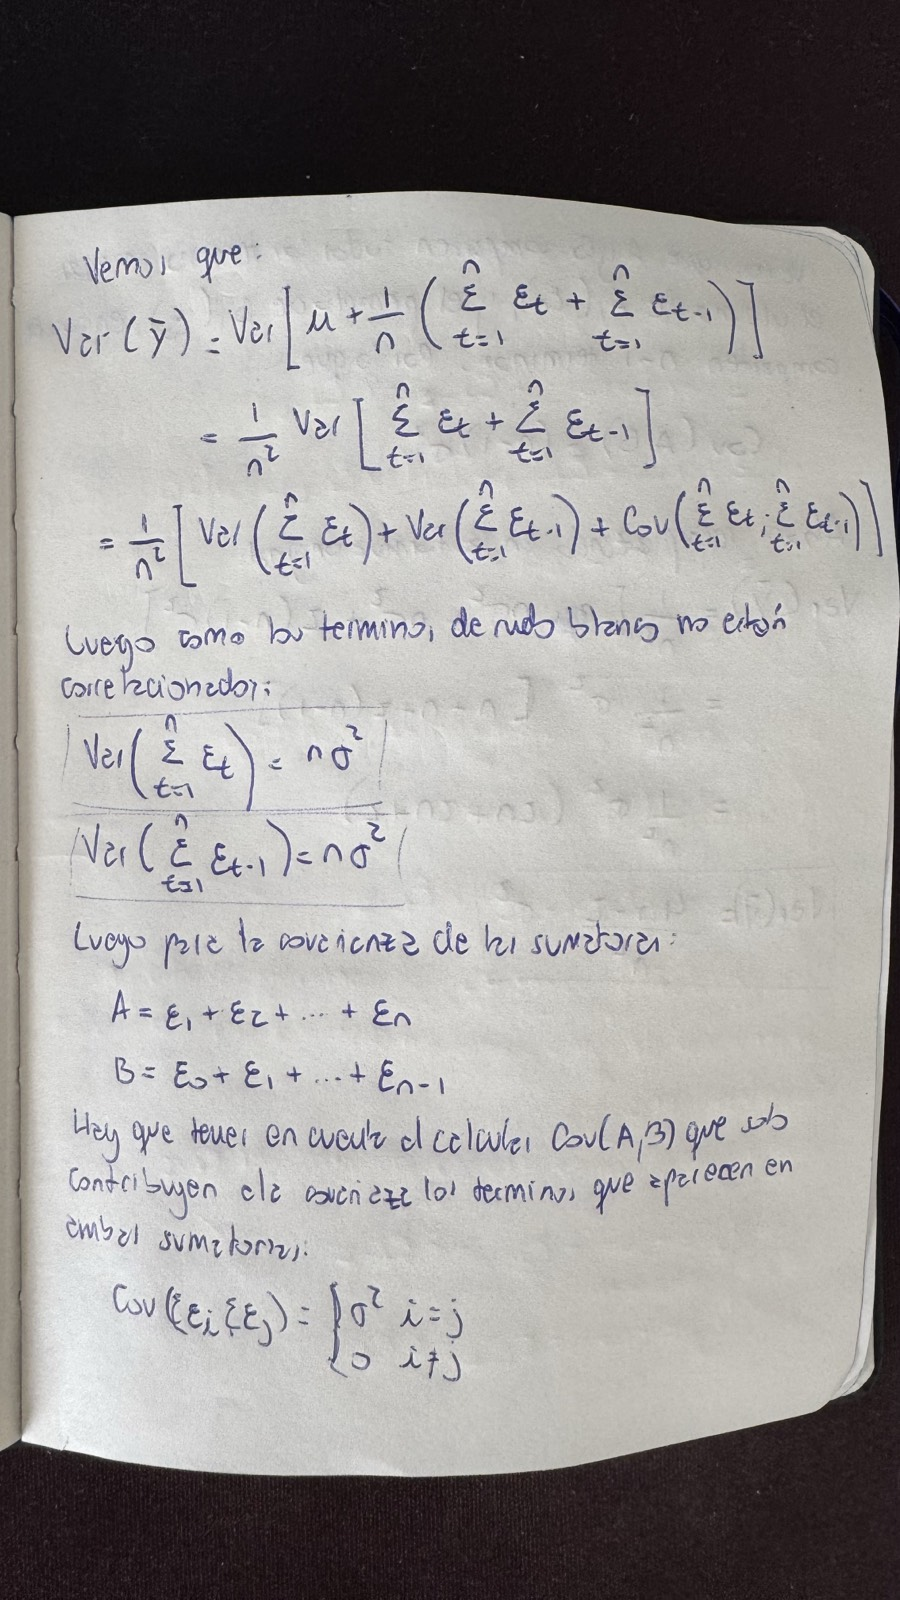
\includegraphics[height=0.86\textheight]{anexo/ej2_pag2.jpg}
\end{center}
\clearpage

\begin{center}
Ejercicio 2, página 3\\[1ex]
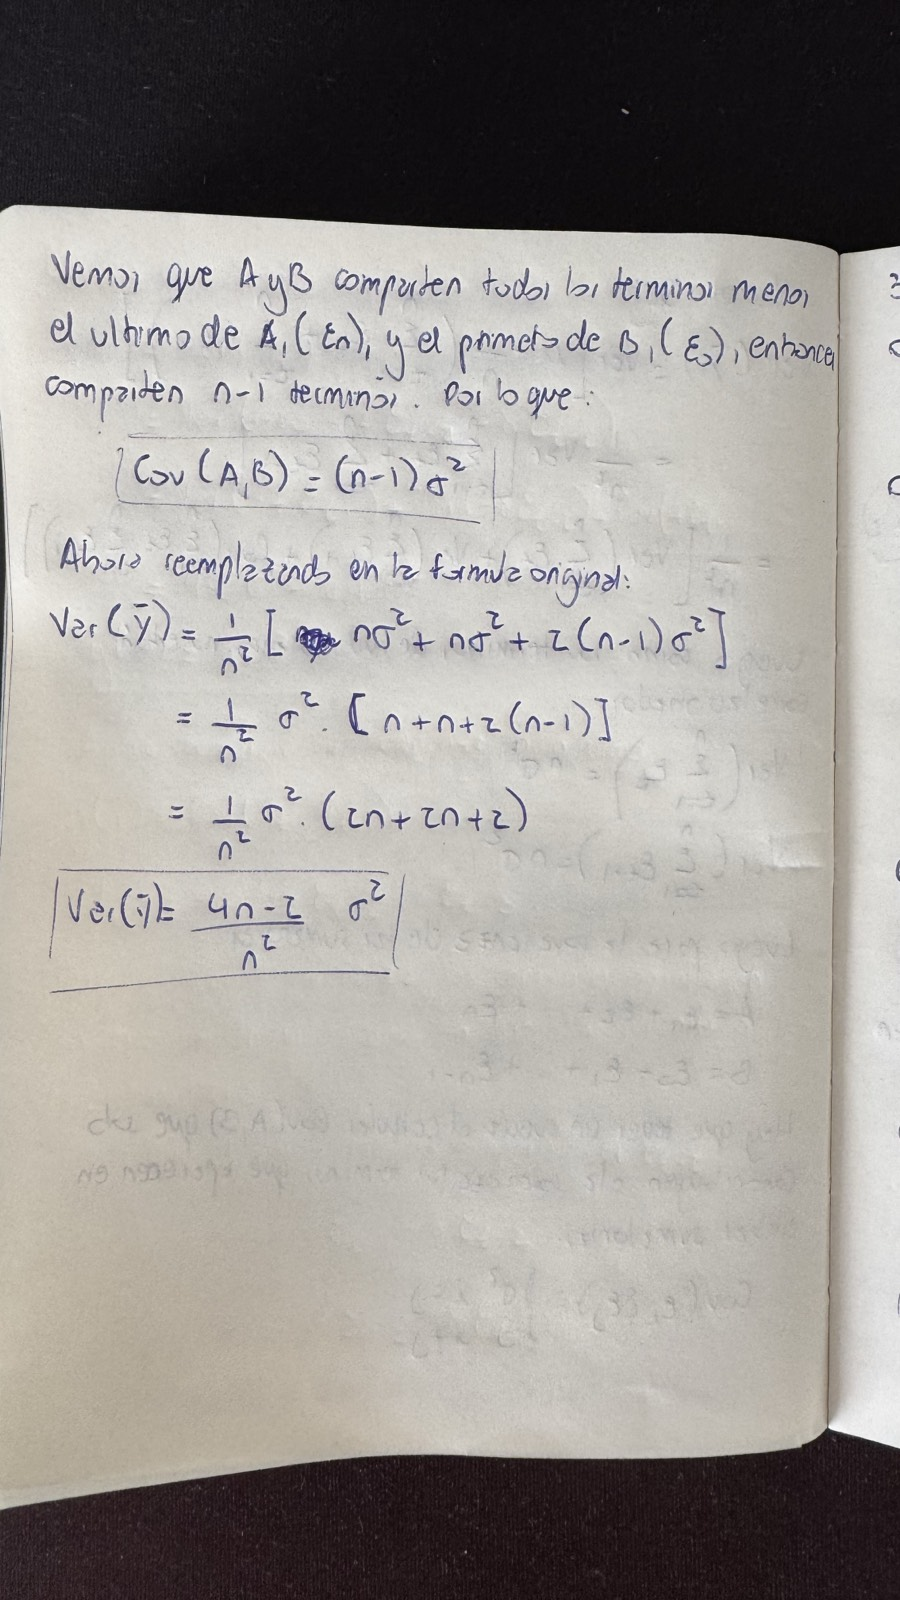
\includegraphics[height=0.86\textheight]{anexo/ej2_pag3.jpg}
\end{center}
\clearpage

\begin{center}
Ejercicio 3, página 1\\[1ex]
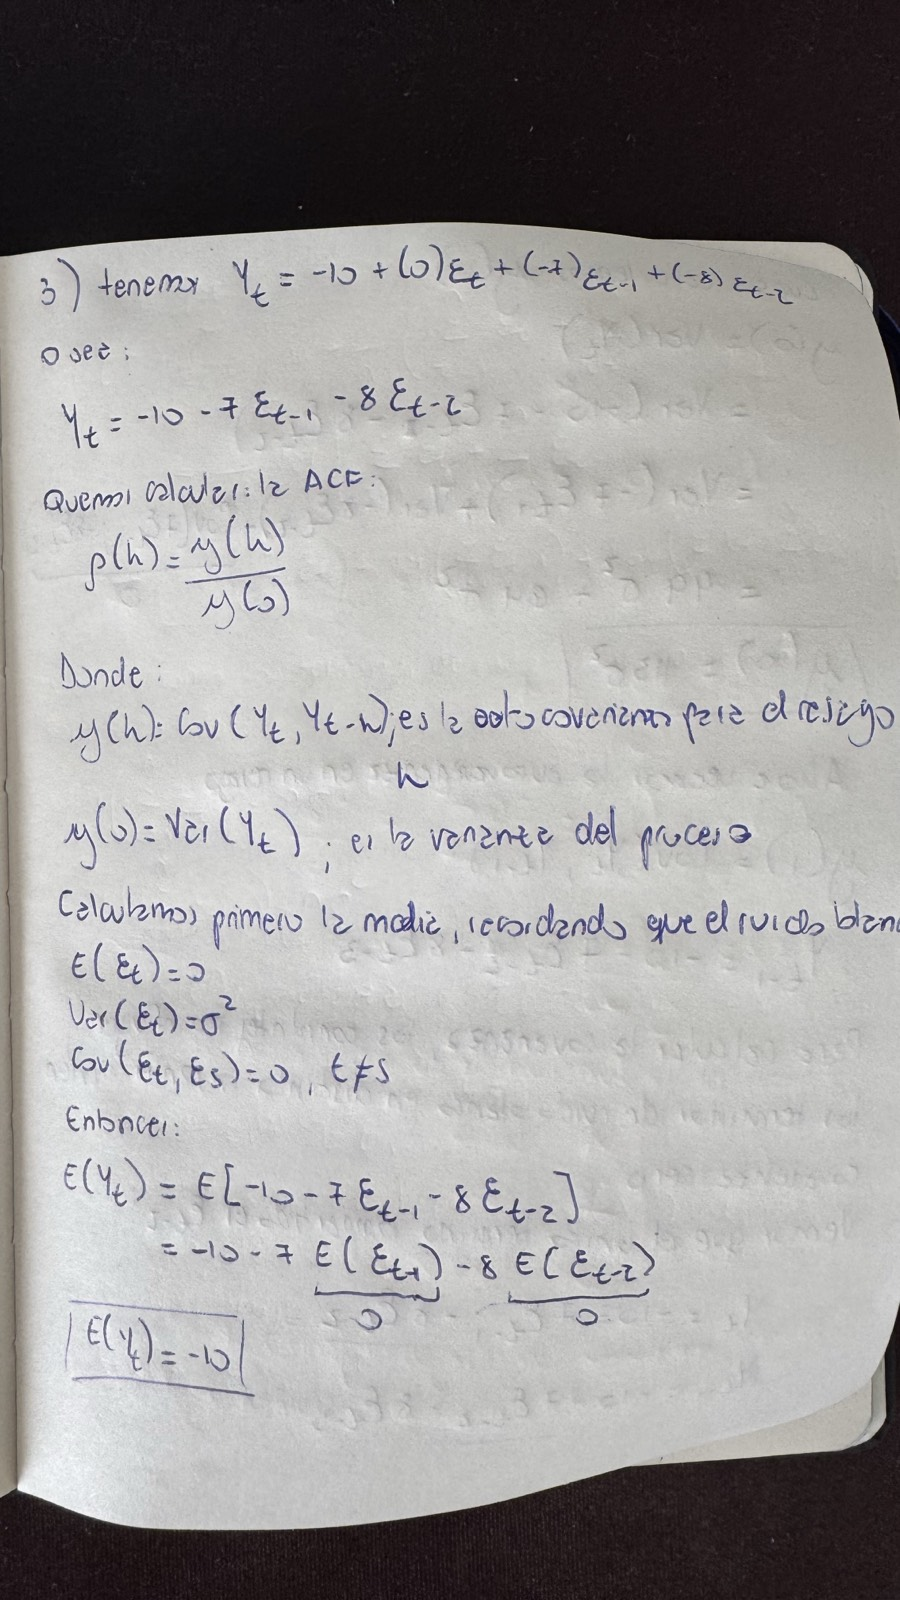
\includegraphics[height=0.86\textheight]{anexo/ej3_pag1.jpg}
\end{center}
\clearpage

\begin{center}
Ejercicio 3, página 2\\[1ex]
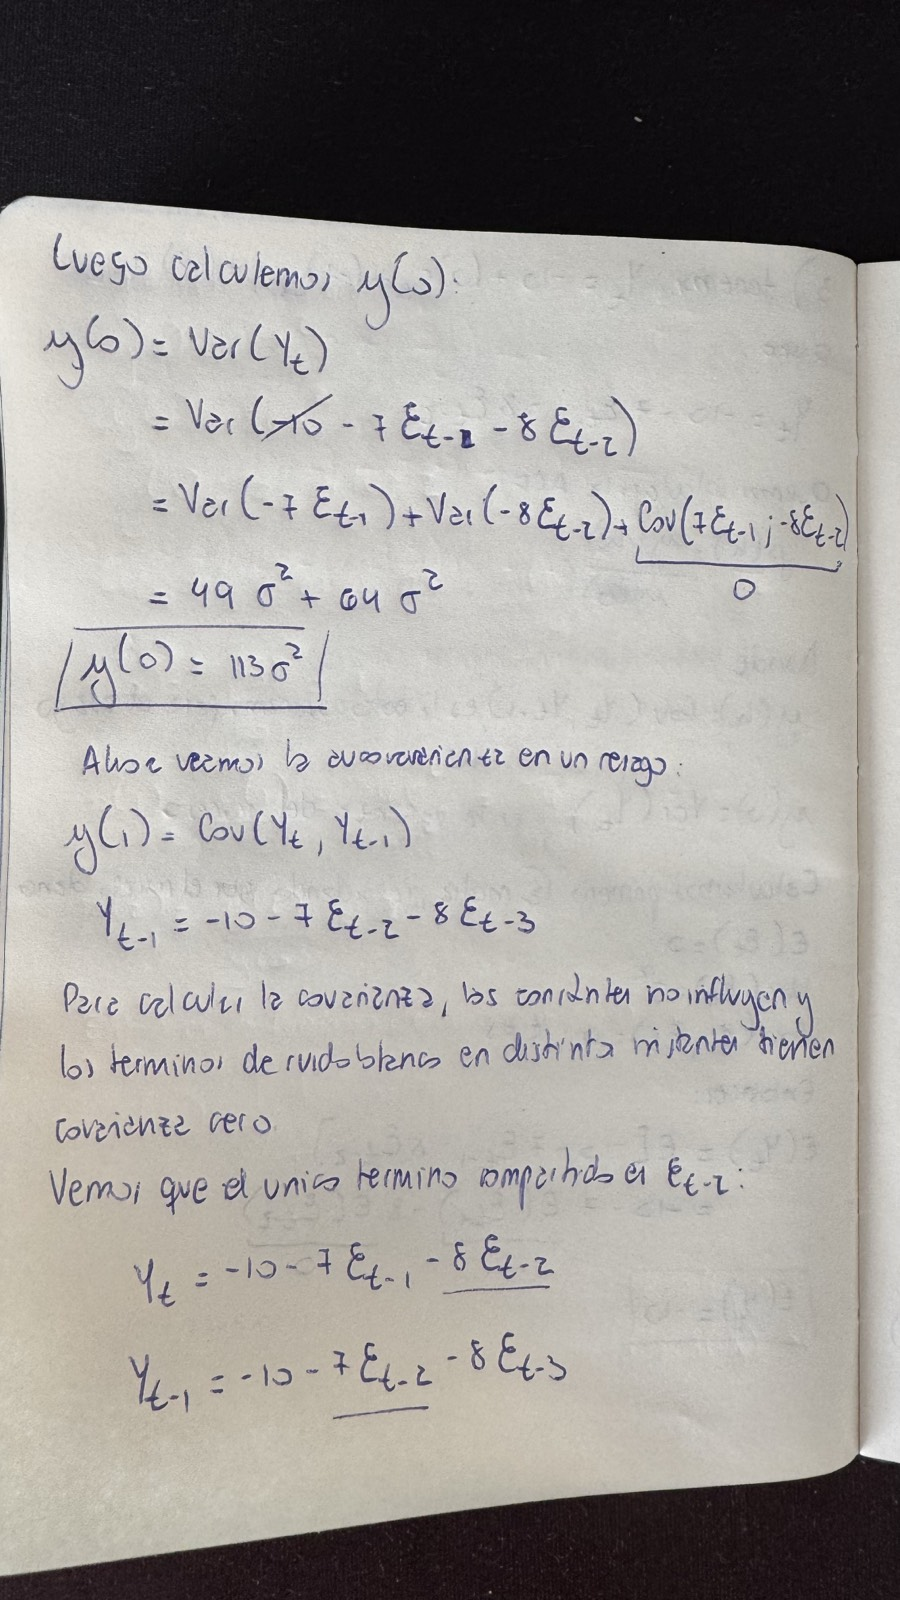
\includegraphics[height=0.86\textheight]{anexo/ej3_pag2.jpg}
\end{center}
\clearpage

\begin{center}
Ejercicio 3, página 3\\[1ex]
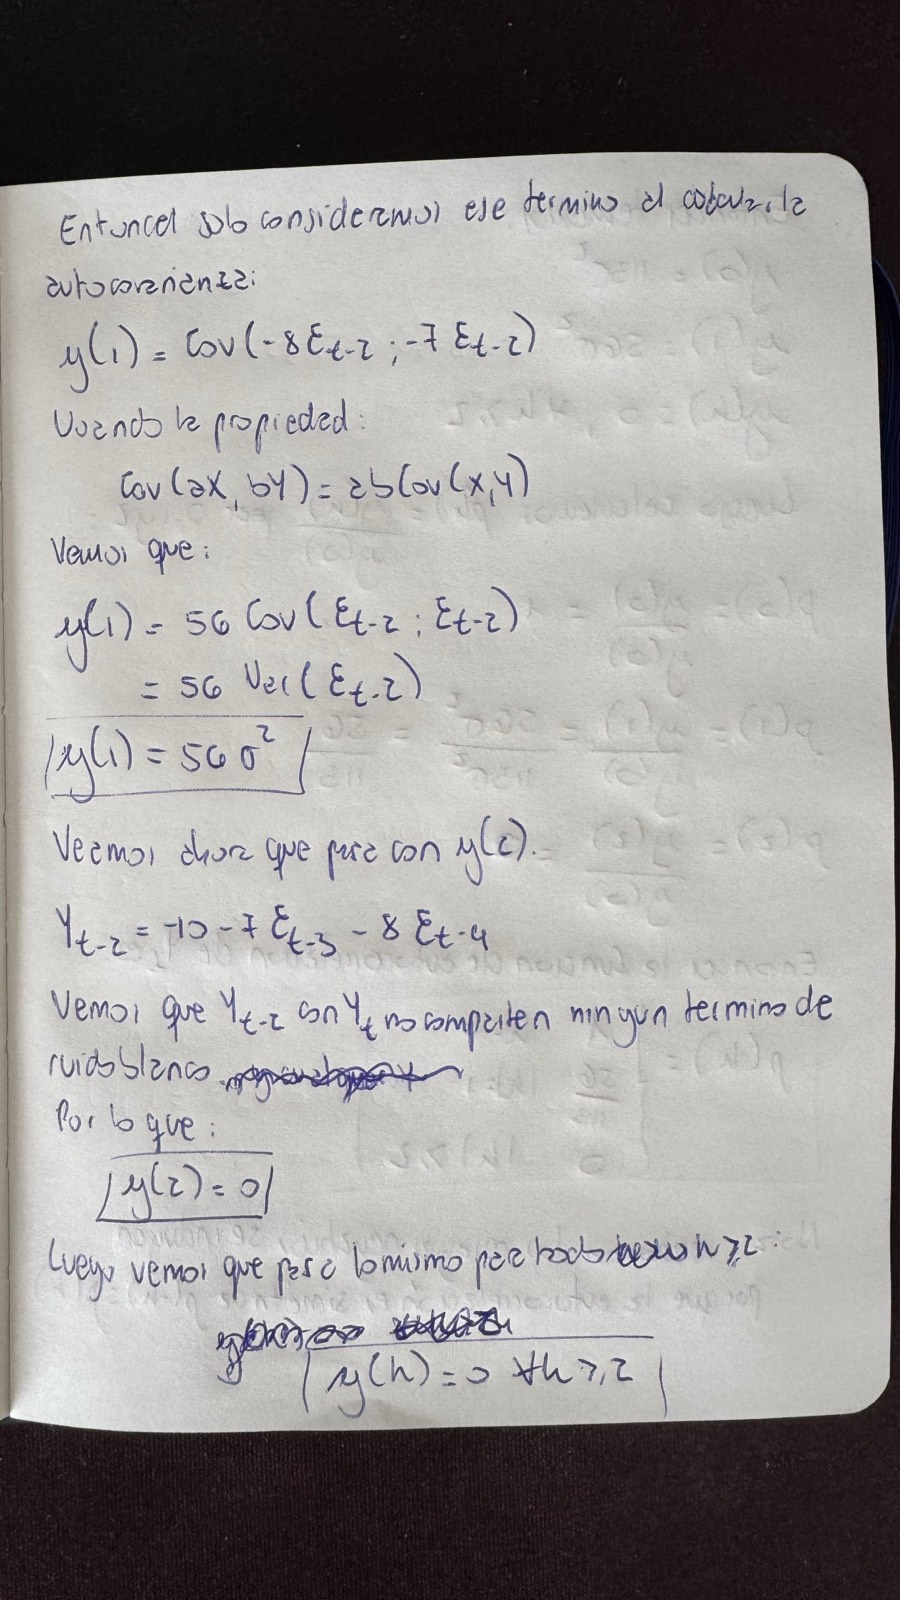
\includegraphics[height=0.86\textheight]{anexo/ej3_pag3.jpg}
\end{center}
\clearpage

\begin{center}
Ejercicio 3, página 4\\[1ex]
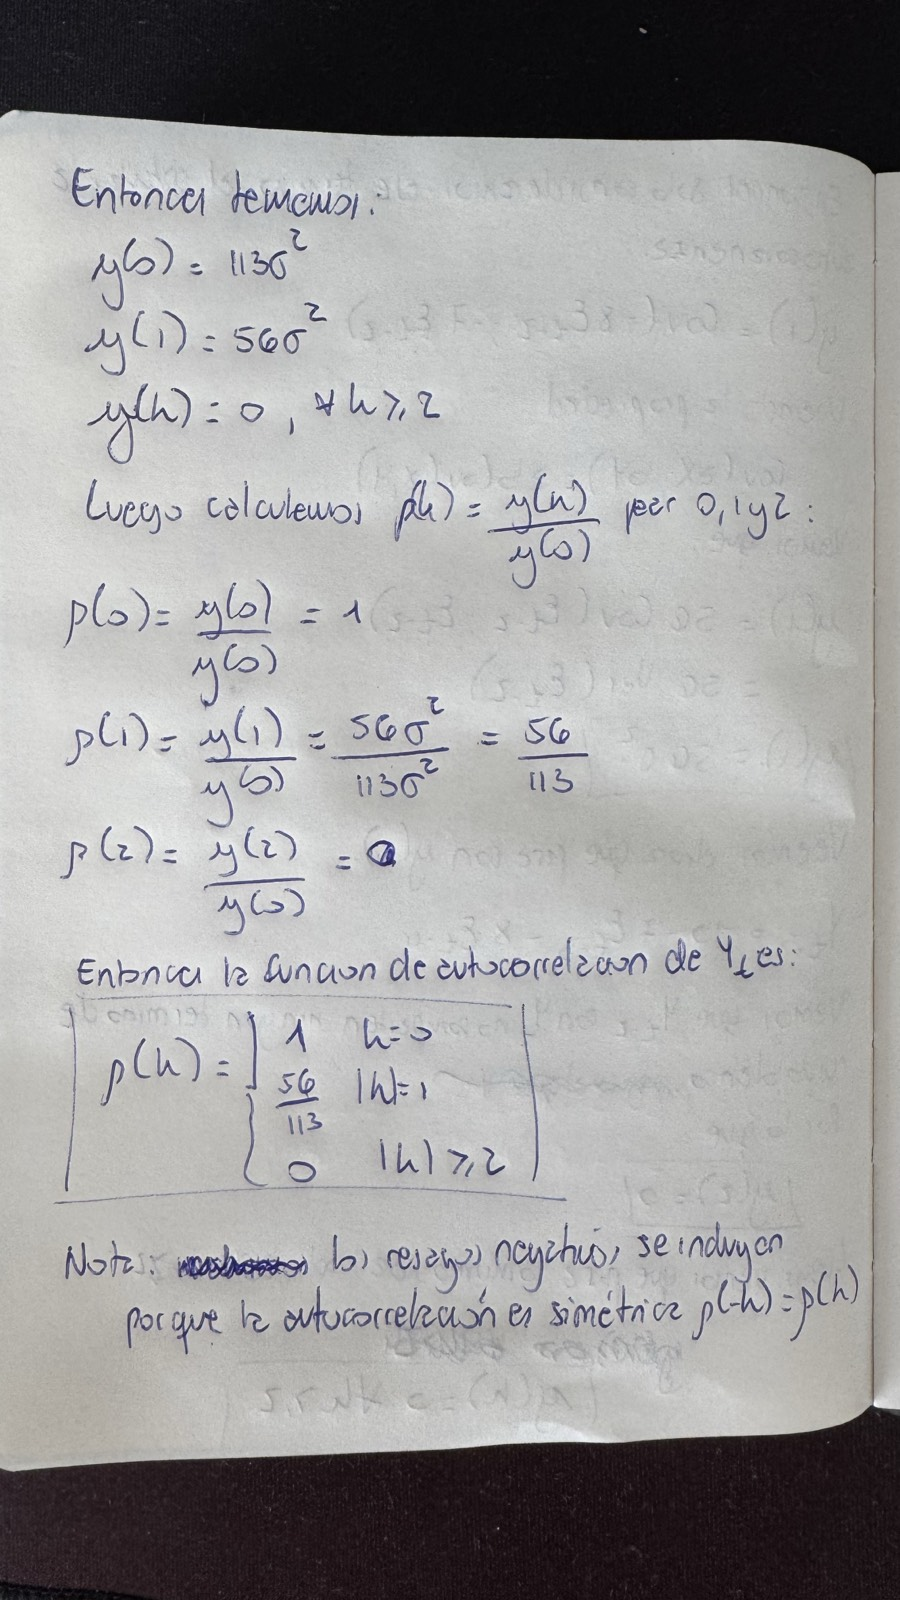
\includegraphics[height=0.86\textheight]{anexo/ej3_pag4.jpg}
\end{center}
\clearpage

\end{document}
